\documentclass[twoside]{book}

% Packages required by doxygen
\usepackage{fixltx2e}
\usepackage{calc}
\usepackage{doxygen}
\usepackage[export]{adjustbox} % also loads graphicx
\usepackage{graphicx}
\usepackage[utf8]{inputenc}
\usepackage{makeidx}
\usepackage{multicol}
\usepackage{multirow}
\PassOptionsToPackage{warn}{textcomp}
\usepackage{textcomp}
\usepackage[nointegrals]{wasysym}
\usepackage[table]{xcolor}

% Font selection
\usepackage[T1]{fontenc}
\usepackage[scaled=.90]{helvet}
\usepackage{courier}
\usepackage{amssymb}
\usepackage{sectsty}
\renewcommand{\familydefault}{\sfdefault}
\allsectionsfont{%
  \fontseries{bc}\selectfont%
  \color{darkgray}%
}
\renewcommand{\DoxyLabelFont}{%
  \fontseries{bc}\selectfont%
  \color{darkgray}%
}
\newcommand{\+}{\discretionary{\mbox{\scriptsize$\hookleftarrow$}}{}{}}

% Page & text layout
\usepackage{geometry}
\geometry{%
  a4paper,%
  top=2.5cm,%
  bottom=2.5cm,%
  left=2.5cm,%
  right=2.5cm%
}
\tolerance=750
\hfuzz=15pt
\hbadness=750
\setlength{\emergencystretch}{15pt}
\setlength{\parindent}{0cm}
\setlength{\parskip}{3ex plus 2ex minus 2ex}
\makeatletter
\renewcommand{\paragraph}{%
  \@startsection{paragraph}{4}{0ex}{-1.0ex}{1.0ex}{%
    \normalfont\normalsize\bfseries\SS@parafont%
  }%
}
\renewcommand{\subparagraph}{%
  \@startsection{subparagraph}{5}{0ex}{-1.0ex}{1.0ex}{%
    \normalfont\normalsize\bfseries\SS@subparafont%
  }%
}
\makeatother

% Headers & footers
\usepackage{fancyhdr}
\pagestyle{fancyplain}
\fancyhead[LE]{\fancyplain{}{\bfseries\thepage}}
\fancyhead[CE]{\fancyplain{}{}}
\fancyhead[RE]{\fancyplain{}{\bfseries\leftmark}}
\fancyhead[LO]{\fancyplain{}{\bfseries\rightmark}}
\fancyhead[CO]{\fancyplain{}{}}
\fancyhead[RO]{\fancyplain{}{\bfseries\thepage}}
\fancyfoot[LE]{\fancyplain{}{}}
\fancyfoot[CE]{\fancyplain{}{}}
\fancyfoot[RE]{\fancyplain{}{\bfseries\scriptsize Generated by Doxygen }}
\fancyfoot[LO]{\fancyplain{}{\bfseries\scriptsize Generated by Doxygen }}
\fancyfoot[CO]{\fancyplain{}{}}
\fancyfoot[RO]{\fancyplain{}{}}
\renewcommand{\footrulewidth}{0.4pt}
\renewcommand{\chaptermark}[1]{%
  \markboth{#1}{}%
}
\renewcommand{\sectionmark}[1]{%
  \markright{\thesection\ #1}%
}

% Indices & bibliography
\usepackage{natbib}
\usepackage[titles]{tocloft}
\setcounter{tocdepth}{3}
\setcounter{secnumdepth}{5}
\makeindex

% Hyperlinks (required, but should be loaded last)
\usepackage{ifpdf}
\ifpdf
  \usepackage[pdftex,pagebackref=true]{hyperref}
\else
  \usepackage[ps2pdf,pagebackref=true]{hyperref}
\fi
\hypersetup{%
  colorlinks=true,%
  linkcolor=blue,%
  citecolor=blue,%
  unicode%
}

% Custom commands
\newcommand{\clearemptydoublepage}{%
  \newpage{\pagestyle{empty}\cleardoublepage}%
}

\usepackage{caption}
\captionsetup{labelsep=space,justification=centering,font={bf},singlelinecheck=off,skip=4pt,position=top}

%===== C O N T E N T S =====

\begin{document}

% Titlepage & ToC
\hypersetup{pageanchor=false,
             bookmarksnumbered=true,
             pdfencoding=unicode
            }
\pagenumbering{alph}
\begin{titlepage}
\vspace*{7cm}
\begin{center}%
{\Large Kommandos }\\
\vspace*{1cm}
{\large Generated by Doxygen 1.8.14}\\
\end{center}
\end{titlepage}
\clearemptydoublepage
\pagenumbering{roman}
\tableofcontents
\clearemptydoublepage
\pagenumbering{arabic}
\hypersetup{pageanchor=true}

%--- Begin generated contents ---
\chapter{Hierarchical Index}
\section{Class Hierarchy}
This inheritance list is sorted roughly, but not completely, alphabetically\-:\begin{DoxyCompactList}
\item \contentsline{section}{Catch\-:\-:Detail\-:\-:Approx}{\pageref{class_catch_1_1_detail_1_1_approx}}{}
\item \contentsline{section}{Catch\-:\-:Assertion\-Handler}{\pageref{class_catch_1_1_assertion_handler}}{}
\item \contentsline{section}{Catch\-:\-:Assertion\-Info}{\pageref{struct_catch_1_1_assertion_info}}{}
\item \contentsline{section}{Catch\-:\-:Assertion\-Reaction}{\pageref{struct_catch_1_1_assertion_reaction}}{}
\item \contentsline{section}{Catch\-:\-:Benchmark\-Looper}{\pageref{class_catch_1_1_benchmark_looper}}{}
\item \contentsline{section}{Bullet}{\pageref{class_bullet}}{}
\item \contentsline{section}{Bullet\-Pool}{\pageref{class_bullet_pool}}{}
\item \contentsline{section}{Camera}{\pageref{class_camera}}{}
\item \contentsline{section}{Catch\-:\-:Matchers\-:\-:Std\-String\-:\-:Cased\-String}{\pageref{struct_catch_1_1_matchers_1_1_std_string_1_1_cased_string}}{}
\item \contentsline{section}{Catch\-:\-:Case\-Sensitive}{\pageref{struct_catch_1_1_case_sensitive}}{}
\item \contentsline{section}{Catch\-\_\-global\-\_\-namespace\-\_\-dummy}{\pageref{struct_catch__global__namespace__dummy}}{}
\item \contentsline{section}{Collision}{\pageref{class_collision}}{}
\item \contentsline{section}{Catch\-:\-:Counts}{\pageref{struct_catch_1_1_counts}}{}
\item \contentsline{section}{Catch\-:\-:Decomposer}{\pageref{struct_catch_1_1_decomposer}}{}
\item \contentsline{section}{Enemy}{\pageref{class_enemy}}{}
\item \contentsline{section}{Enemy\-Pool}{\pageref{class_enemy_pool}}{}
\item \contentsline{section}{Enemy\-Spawner}{\pageref{class_enemy_spawner}}{}
\item \contentsline{section}{Catch\-:\-:Exception\-Translator\-Registrar}{\pageref{class_catch_1_1_exception_translator_registrar}}{}
\item \contentsline{section}{Catch\-:\-:Expr\-Lhs$<$ Lhs\-T $>$}{\pageref{class_catch_1_1_expr_lhs}}{}
\item \contentsline{section}{Game}{\pageref{class_game}}{}
\item \contentsline{section}{Game\-Over\-State}{\pageref{class_game_over_state}}{}
\item \contentsline{section}{Heat\-Map\-Manager}{\pageref{class_heat_map_manager}}{}
\item I\-Event\-Receiver\begin{DoxyCompactList}
\item \contentsline{section}{Input\-Receiver}{\pageref{class_input_receiver}}{}
\end{DoxyCompactList}
\item \contentsline{section}{Catch\-:\-:I\-Exception\-Translator}{\pageref{struct_catch_1_1_i_exception_translator}}{}
\begin{DoxyCompactList}
\item \contentsline{section}{Catch\-:\-:Exception\-Translator\-Registrar\-:\-:Exception\-Translator$<$ T $>$}{\pageref{class_catch_1_1_exception_translator_registrar_1_1_exception_translator}}{}
\end{DoxyCompactList}
\item \contentsline{section}{Catch\-:\-:I\-Exception\-Translator\-Registry}{\pageref{struct_catch_1_1_i_exception_translator_registry}}{}
\item \contentsline{section}{Catch\-:\-:I\-Mutable\-Registry\-Hub}{\pageref{struct_catch_1_1_i_mutable_registry_hub}}{}
\item \contentsline{section}{Catch\-:\-:I\-Registry\-Hub}{\pageref{struct_catch_1_1_i_registry_hub}}{}
\item \contentsline{section}{Catch\-:\-:I\-Result\-Capture}{\pageref{struct_catch_1_1_i_result_capture}}{}
\item \contentsline{section}{Catch\-:\-:I\-Runner}{\pageref{struct_catch_1_1_i_runner}}{}
\item \contentsline{section}{Catch\-:\-:is\-\_\-range$<$ T $>$}{\pageref{struct_catch_1_1is__range}}{}
\item \contentsline{section}{Catch\-:\-:Detail\-:\-:Is\-Stream\-Insertable$<$ T $>$}{\pageref{class_catch_1_1_detail_1_1_is_stream_insertable}}{}
\item \contentsline{section}{Catch\-:\-:I\-Stream}{\pageref{struct_catch_1_1_i_stream}}{}
\item \contentsline{section}{Catch\-:\-:I\-Test\-Case\-Registry}{\pageref{struct_catch_1_1_i_test_case_registry}}{}
\item \contentsline{section}{Catch\-:\-:I\-Test\-Invoker}{\pageref{struct_catch_1_1_i_test_invoker}}{}
\begin{DoxyCompactList}
\item \contentsline{section}{Catch\-:\-:Test\-Invoker\-As\-Method$<$ C $>$}{\pageref{class_catch_1_1_test_invoker_as_method}}{}
\end{DoxyCompactList}
\item \contentsline{section}{Catch\-:\-:I\-Transient\-Expression}{\pageref{struct_catch_1_1_i_transient_expression}}{}
\begin{DoxyCompactList}
\item \contentsline{section}{Catch\-:\-:Binary\-Expr$<$ Lhs\-T, Rhs\-T $>$}{\pageref{class_catch_1_1_binary_expr}}{}
\item \contentsline{section}{Catch\-:\-:Match\-Expr$<$ Arg\-T, Matcher\-T $>$}{\pageref{class_catch_1_1_match_expr}}{}
\item \contentsline{section}{Catch\-:\-:Unary\-Expr$<$ Lhs\-T $>$}{\pageref{class_catch_1_1_unary_expr}}{}
\end{DoxyCompactList}
\item \contentsline{section}{Catch\-:\-:Lazy\-Expression}{\pageref{class_catch_1_1_lazy_expression}}{}
\item \contentsline{section}{Catch\-:\-:Matchers\-:\-:Impl\-:\-:Matcher\-Method$<$ Object\-T $>$}{\pageref{struct_catch_1_1_matchers_1_1_impl_1_1_matcher_method}}{}
\item \contentsline{section}{Catch\-:\-:Matchers\-:\-:Impl\-:\-:Matcher\-Method$<$ Arg\-T $>$}{\pageref{struct_catch_1_1_matchers_1_1_impl_1_1_matcher_method}}{}
\begin{DoxyCompactList}
\item \contentsline{section}{Catch\-:\-:Matchers\-:\-:Impl\-:\-:Matcher\-Base$<$ Arg\-T $>$}{\pageref{struct_catch_1_1_matchers_1_1_impl_1_1_matcher_base}}{}
\begin{DoxyCompactList}
\item \contentsline{section}{Catch\-:\-:Matchers\-:\-:Impl\-:\-:Match\-All\-Of$<$ Arg\-T $>$}{\pageref{struct_catch_1_1_matchers_1_1_impl_1_1_match_all_of}}{}
\item \contentsline{section}{Catch\-:\-:Matchers\-:\-:Impl\-:\-:Match\-Any\-Of$<$ Arg\-T $>$}{\pageref{struct_catch_1_1_matchers_1_1_impl_1_1_match_any_of}}{}
\item \contentsline{section}{Catch\-:\-:Matchers\-:\-:Impl\-:\-:Match\-Not\-Of$<$ Arg\-T $>$}{\pageref{struct_catch_1_1_matchers_1_1_impl_1_1_match_not_of}}{}
\end{DoxyCompactList}
\end{DoxyCompactList}
\item \contentsline{section}{Catch\-:\-:Matchers\-:\-:Impl\-:\-:Matcher\-Method$<$ Ptr\-T $\ast$ $>$}{\pageref{struct_catch_1_1_matchers_1_1_impl_1_1_matcher_method_3_01_ptr_t_01_5_01_4}}{}
\item \contentsline{section}{Catch\-:\-:Matchers\-:\-:Impl\-:\-:Matcher\-Method$<$ T $>$}{\pageref{struct_catch_1_1_matchers_1_1_impl_1_1_matcher_method}}{}
\begin{DoxyCompactList}
\item \contentsline{section}{Catch\-:\-:Matchers\-:\-:Impl\-:\-:Matcher\-Base$<$ T $>$}{\pageref{struct_catch_1_1_matchers_1_1_impl_1_1_matcher_base}}{}
\end{DoxyCompactList}
\item \contentsline{section}{Catch\-:\-:Matchers\-:\-:Impl\-:\-:Matcher\-Untyped\-Base}{\pageref{class_catch_1_1_matchers_1_1_impl_1_1_matcher_untyped_base}}{}
\begin{DoxyCompactList}
\item \contentsline{section}{Catch\-:\-:Matchers\-:\-:Impl\-:\-:Matcher\-Base$<$ T $>$}{\pageref{struct_catch_1_1_matchers_1_1_impl_1_1_matcher_base}}{}
\item \contentsline{section}{Catch\-:\-:Matchers\-:\-:Impl\-:\-:Matcher\-Base$<$ Arg\-T $>$}{\pageref{struct_catch_1_1_matchers_1_1_impl_1_1_matcher_base}}{}
\end{DoxyCompactList}
\item \contentsline{section}{Catch\-:\-:Message\-Info}{\pageref{struct_catch_1_1_message_info}}{}
\item \contentsline{section}{Catch\-:\-:Message\-Stream}{\pageref{struct_catch_1_1_message_stream}}{}
\begin{DoxyCompactList}
\item \contentsline{section}{Catch\-:\-:Message\-Builder}{\pageref{struct_catch_1_1_message_builder}}{}
\end{DoxyCompactList}
\item \contentsline{section}{Catch\-:\-:Name\-And\-Tags}{\pageref{struct_catch_1_1_name_and_tags}}{}
\item \contentsline{section}{Catch\-:\-:Non\-Copyable}{\pageref{class_catch_1_1_non_copyable}}{}
\begin{DoxyCompactList}
\item \contentsline{section}{Catch\-:\-:Auto\-Reg}{\pageref{struct_catch_1_1_auto_reg}}{}
\item \contentsline{section}{Catch\-:\-:Section}{\pageref{class_catch_1_1_section}}{}
\end{DoxyCompactList}
\item \contentsline{section}{Catch\-:\-:not\-\_\-this\-\_\-one}{\pageref{struct_catch_1_1not__this__one}}{}
\item \contentsline{section}{Object\-Placement\-Generation}{\pageref{class_object_placement_generation}}{}
\item \contentsline{section}{Particle}{\pageref{struct_particle}}{}
\item \contentsline{section}{Particle\-System}{\pageref{class_particle_system}}{}
\item \contentsline{section}{Player}{\pageref{class_player}}{}
\item \contentsline{section}{Catch\-:\-:pluralise}{\pageref{struct_catch_1_1pluralise}}{}
\item \contentsline{section}{Powerup}{\pageref{class_powerup}}{}
\item \contentsline{section}{Powerup\-Pool}{\pageref{class_powerup_pool}}{}
\item \contentsline{section}{Power\-Up\-Spawner}{\pageref{class_power_up_spawner}}{}
\item \contentsline{section}{Catch\-:\-:Registrar\-For\-Tag\-Aliases}{\pageref{struct_catch_1_1_registrar_for_tag_aliases}}{}
\item \contentsline{section}{Catch\-:\-:Result\-Disposition}{\pageref{struct_catch_1_1_result_disposition}}{}
\item \contentsline{section}{Catch\-:\-:Result\-Was}{\pageref{struct_catch_1_1_result_was}}{}
\item \contentsline{section}{Catch\-:\-:Reusable\-String\-Stream}{\pageref{class_catch_1_1_reusable_string_stream}}{}
\item \contentsline{section}{Catch\-:\-:Scoped\-Message}{\pageref{class_catch_1_1_scoped_message}}{}
\item \contentsline{section}{Score}{\pageref{class_score}}{}
\item \contentsline{section}{Catch\-:\-:Section\-End\-Info}{\pageref{struct_catch_1_1_section_end_info}}{}
\item \contentsline{section}{Catch\-:\-:Section\-Info}{\pageref{struct_catch_1_1_section_info}}{}
\item \contentsline{section}{Sound\-Manager}{\pageref{class_sound_manager}}{}
\item \contentsline{section}{Catch\-:\-:Source\-Line\-Info}{\pageref{struct_catch_1_1_source_line_info}}{}
\item \contentsline{section}{Catch\-:\-:Stream\-End\-Stop}{\pageref{struct_catch_1_1_stream_end_stop}}{}
\item \contentsline{section}{Catch\-:\-:String\-Maker$<$ T, typename $>$}{\pageref{struct_catch_1_1_string_maker}}{}
\item \contentsline{section}{Catch\-:\-:String\-Maker$<$ bool $>$}{\pageref{struct_catch_1_1_string_maker_3_01bool_01_4}}{}
\item \contentsline{section}{Catch\-:\-:String\-Maker$<$ Catch\-:\-:Detail\-:\-:Approx $>$}{\pageref{struct_catch_1_1_string_maker_3_01_catch_1_1_detail_1_1_approx_01_4}}{}
\item \contentsline{section}{Catch\-:\-:String\-Maker$<$ char $\ast$ $>$}{\pageref{struct_catch_1_1_string_maker_3_01char_01_5_01_4}}{}
\item \contentsline{section}{Catch\-:\-:String\-Maker$<$ char $>$}{\pageref{struct_catch_1_1_string_maker_3_01char_01_4}}{}
\item \contentsline{section}{Catch\-:\-:String\-Maker$<$ char const $\ast$ $>$}{\pageref{struct_catch_1_1_string_maker_3_01char_01const_01_5_01_4}}{}
\item \contentsline{section}{Catch\-:\-:String\-Maker$<$ char\mbox{[}S\-Z\mbox{]}$>$}{\pageref{struct_catch_1_1_string_maker_3_01char[_s_z]_4}}{}
\item \contentsline{section}{Catch\-:\-:String\-Maker$<$ double $>$}{\pageref{struct_catch_1_1_string_maker_3_01double_01_4}}{}
\item \contentsline{section}{Catch\-:\-:String\-Maker$<$ float $>$}{\pageref{struct_catch_1_1_string_maker_3_01float_01_4}}{}
\item \contentsline{section}{Catch\-:\-:String\-Maker$<$ int $>$}{\pageref{struct_catch_1_1_string_maker_3_01int_01_4}}{}
\item \contentsline{section}{Catch\-:\-:String\-Maker$<$ long $>$}{\pageref{struct_catch_1_1_string_maker_3_01long_01_4}}{}
\item \contentsline{section}{Catch\-:\-:String\-Maker$<$ long long $>$}{\pageref{struct_catch_1_1_string_maker_3_01long_01long_01_4}}{}
\item \contentsline{section}{Catch\-:\-:String\-Maker$<$ R C\-:\-:$\ast$ $>$}{\pageref{struct_catch_1_1_string_maker_3_01_r_01_c_1_1_5_01_4}}{}
\item \contentsline{section}{Catch\-:\-:String\-Maker$<$ R, typename std\-:\-:enable\-\_\-if$<$ is\-\_\-range$<$ R $>$\-:\-:value \&\&!\-:\-:Catch\-:\-:Detail\-:\-:Is\-Stream\-Insertable$<$ R $>$\-:\-:value $>$\-:\-:type $>$}{\pageref{struct_catch_1_1_string_maker_3_01_r_00_01typename_01std_1_1enable__if_3_01is__range_3_01_r_01_4536d8fedfff6d62432b3dc59b56e1380}}{}
\item \contentsline{section}{Catch\-:\-:String\-Maker$<$ signed char $>$}{\pageref{struct_catch_1_1_string_maker_3_01signed_01char_01_4}}{}
\item \contentsline{section}{Catch\-:\-:String\-Maker$<$ signed char\mbox{[}S\-Z\mbox{]}$>$}{\pageref{struct_catch_1_1_string_maker_3_01signed_01char[_s_z]_4}}{}
\item \contentsline{section}{Catch\-:\-:String\-Maker$<$ std\-:\-:nullptr\-\_\-t $>$}{\pageref{struct_catch_1_1_string_maker_3_01std_1_1nullptr__t_01_4}}{}
\item \contentsline{section}{Catch\-:\-:String\-Maker$<$ std\-:\-:string $>$}{\pageref{struct_catch_1_1_string_maker_3_01std_1_1string_01_4}}{}
\item \contentsline{section}{Catch\-:\-:String\-Maker$<$ std\-:\-:wstring $>$}{\pageref{struct_catch_1_1_string_maker_3_01std_1_1wstring_01_4}}{}
\item \contentsline{section}{Catch\-:\-:String\-Maker$<$ T $\ast$ $>$}{\pageref{struct_catch_1_1_string_maker_3_01_t_01_5_01_4}}{}
\item \contentsline{section}{Catch\-:\-:String\-Maker$<$ T\mbox{[}S\-Z\mbox{]}$>$}{\pageref{struct_catch_1_1_string_maker_3_01_t[_s_z]_4}}{}
\item \contentsline{section}{Catch\-:\-:String\-Maker$<$ unsigned char $>$}{\pageref{struct_catch_1_1_string_maker_3_01unsigned_01char_01_4}}{}
\item \contentsline{section}{Catch\-:\-:String\-Maker$<$ unsigned char\mbox{[}S\-Z\mbox{]}$>$}{\pageref{struct_catch_1_1_string_maker_3_01unsigned_01char[_s_z]_4}}{}
\item \contentsline{section}{Catch\-:\-:String\-Maker$<$ unsigned int $>$}{\pageref{struct_catch_1_1_string_maker_3_01unsigned_01int_01_4}}{}
\item \contentsline{section}{Catch\-:\-:String\-Maker$<$ unsigned long $>$}{\pageref{struct_catch_1_1_string_maker_3_01unsigned_01long_01_4}}{}
\item \contentsline{section}{Catch\-:\-:String\-Maker$<$ unsigned long long $>$}{\pageref{struct_catch_1_1_string_maker_3_01unsigned_01long_01long_01_4}}{}
\item \contentsline{section}{Catch\-:\-:String\-Maker$<$ wchar\-\_\-t $\ast$ $>$}{\pageref{struct_catch_1_1_string_maker_3_01wchar__t_01_5_01_4}}{}
\item \contentsline{section}{Catch\-:\-:String\-Maker$<$ wchar\-\_\-t const $\ast$ $>$}{\pageref{struct_catch_1_1_string_maker_3_01wchar__t_01const_01_5_01_4}}{}
\item \contentsline{section}{Catch\-:\-:String\-Ref}{\pageref{class_catch_1_1_string_ref}}{}
\item \contentsline{section}{Catch\-:\-:Test\-Case\-Info}{\pageref{struct_catch_1_1_test_case_info}}{}
\begin{DoxyCompactList}
\item \contentsline{section}{Catch\-:\-:Test\-Case}{\pageref{class_catch_1_1_test_case}}{}
\end{DoxyCompactList}
\item \contentsline{section}{Catch\-:\-:Test\-Failure\-Exception}{\pageref{struct_catch_1_1_test_failure_exception}}{}
\item \contentsline{section}{Catch\-:\-:Timer}{\pageref{class_catch_1_1_timer}}{}
\item \contentsline{section}{Catch\-:\-:Totals}{\pageref{struct_catch_1_1_totals}}{}
\item \contentsline{section}{Tutorial}{\pageref{class_tutorial}}{}
\item \contentsline{section}{U\-I\-System}{\pageref{class_u_i_system}}{}
\item \contentsline{section}{Wave\-Data}{\pageref{struct_wave_data}}{}
\item Matcher\-Base\begin{DoxyCompactList}
\item \contentsline{section}{Catch\-:\-:Matchers\-:\-:Floating\-:\-:Within\-Abs\-Matcher}{\pageref{struct_catch_1_1_matchers_1_1_floating_1_1_within_abs_matcher}}{}
\item \contentsline{section}{Catch\-:\-:Matchers\-:\-:Floating\-:\-:Within\-Ulps\-Matcher}{\pageref{struct_catch_1_1_matchers_1_1_floating_1_1_within_ulps_matcher}}{}
\item \contentsline{section}{Catch\-:\-:Matchers\-:\-:Generic\-:\-:Predicate\-Matcher$<$ T $>$}{\pageref{class_catch_1_1_matchers_1_1_generic_1_1_predicate_matcher}}{}
\item \contentsline{section}{Catch\-:\-:Matchers\-:\-:Std\-String\-:\-:Regex\-Matcher}{\pageref{struct_catch_1_1_matchers_1_1_std_string_1_1_regex_matcher}}{}
\item \contentsline{section}{Catch\-:\-:Matchers\-:\-:Std\-String\-:\-:String\-Matcher\-Base}{\pageref{struct_catch_1_1_matchers_1_1_std_string_1_1_string_matcher_base}}{}
\begin{DoxyCompactList}
\item \contentsline{section}{Catch\-:\-:Matchers\-:\-:Std\-String\-:\-:Contains\-Matcher}{\pageref{struct_catch_1_1_matchers_1_1_std_string_1_1_contains_matcher}}{}
\item \contentsline{section}{Catch\-:\-:Matchers\-:\-:Std\-String\-:\-:Ends\-With\-Matcher}{\pageref{struct_catch_1_1_matchers_1_1_std_string_1_1_ends_with_matcher}}{}
\item \contentsline{section}{Catch\-:\-:Matchers\-:\-:Std\-String\-:\-:Equals\-Matcher}{\pageref{struct_catch_1_1_matchers_1_1_std_string_1_1_equals_matcher}}{}
\item \contentsline{section}{Catch\-:\-:Matchers\-:\-:Std\-String\-:\-:Starts\-With\-Matcher}{\pageref{struct_catch_1_1_matchers_1_1_std_string_1_1_starts_with_matcher}}{}
\end{DoxyCompactList}
\item \contentsline{section}{Catch\-:\-:Matchers\-:\-:Vector\-:\-:Contains\-Element\-Matcher$<$ T $>$}{\pageref{struct_catch_1_1_matchers_1_1_vector_1_1_contains_element_matcher}}{}
\item \contentsline{section}{Catch\-:\-:Matchers\-:\-:Vector\-:\-:Contains\-Matcher$<$ T $>$}{\pageref{struct_catch_1_1_matchers_1_1_vector_1_1_contains_matcher}}{}
\item \contentsline{section}{Catch\-:\-:Matchers\-:\-:Vector\-:\-:Equals\-Matcher$<$ T $>$}{\pageref{struct_catch_1_1_matchers_1_1_vector_1_1_equals_matcher}}{}
\item \contentsline{section}{Catch\-:\-:Matchers\-:\-:Vector\-:\-:Unordered\-Equals\-Matcher$<$ T $>$}{\pageref{struct_catch_1_1_matchers_1_1_vector_1_1_unordered_equals_matcher}}{}
\end{DoxyCompactList}
\end{DoxyCompactList}

\chapter{Class Index}
\section{Class List}
Here are the classes, structs, unions and interfaces with brief descriptions\+:\begin{DoxyCompactList}
\item\contentsline{section}{\mbox{\hyperlink{class_collision}{Collision}} }{\pageref{class_collision}}{}
\item\contentsline{section}{\mbox{\hyperlink{class_enemy_behaviour}{Enemy\+Behaviour}} }{\pageref{class_enemy_behaviour}}{}
\item\contentsline{section}{\mbox{\hyperlink{class_game_over_state}{Game\+Over\+State}} }{\pageref{class_game_over_state}}{}
\item\contentsline{section}{\mbox{\hyperlink{class_input_receiver}{Input\+Receiver}} }{\pageref{class_input_receiver}}{}
\item\contentsline{section}{\mbox{\hyperlink{class_level_generation}{Level\+Generation}} }{\pageref{class_level_generation}}{}
\item\contentsline{section}{\mbox{\hyperlink{class_player}{Player}} }{\pageref{class_player}}{}
\end{DoxyCompactList}

\chapter{Class Documentation}
\hypertarget{class_collision}{}\section{Collision Class Reference}
\label{class_collision}\index{Collision@{Collision}}
\subsection*{Public Member Functions}
\begin{DoxyCompactItemize}
\item 
\mbox{\Hypertarget{class_collision_aa2fa3418899ac7948b31eb909dea6f04}\label{class_collision_aa2fa3418899ac7948b31eb909dea6f04}} 
bool {\bfseries Scene\+Node\+With\+Scene\+Node} (irr\+::scene\+::\+I\+Scene\+Node $\ast$t\+Box1, irr\+::scene\+::\+I\+Scene\+Node $\ast$t\+Box2)
\item 
\mbox{\Hypertarget{class_collision_a673528880f1ad75dab13a2107a3d2b7c}\label{class_collision_a673528880f1ad75dab13a2107a3d2b7c}} 
void {\bfseries Add\+Static\+To\+List} (irr\+::scene\+::\+I\+Scene\+Node $\ast$static\+Object)
\item 
\mbox{\Hypertarget{class_collision_a334467ec1c8b7889aa46016fcedb13f9}\label{class_collision_a334467ec1c8b7889aa46016fcedb13f9}} 
bool {\bfseries Collides\+With\+Static\+Objects} (irr\+::scene\+::\+I\+Scene\+Node $\ast$dynamic\+Object)
\end{DoxyCompactItemize}


The documentation for this class was generated from the following files\+:\begin{DoxyCompactItemize}
\item 
D\+:/\+Documenten/\+S\+T\+U\+D\+I\+E G\+D/\+Game Engine/\+Irrlicht project/kommandos/Collision.\+h\item 
D\+:/\+Documenten/\+S\+T\+U\+D\+I\+E G\+D/\+Game Engine/\+Irrlicht project/kommandos/Collision.\+cpp\end{DoxyCompactItemize}

\hypertarget{class_enemy_behaviour}{}\section{Enemy\+Behaviour Class Reference}
\label{class_enemy_behaviour}\index{Enemy\+Behaviour@{Enemy\+Behaviour}}
\subsection*{Public Member Functions}
\begin{DoxyCompactItemize}
\item 
\mbox{\Hypertarget{class_enemy_behaviour_ab939353a2a71b7845ab189c513428261}\label{class_enemy_behaviour_ab939353a2a71b7845ab189c513428261}} 
I\+Mesh\+Scene\+Node $\ast$ {\bfseries Spawn} (Irrlicht\+Device $\ast$device, vector3df start\+Position)
\item 
\mbox{\Hypertarget{class_enemy_behaviour_a1d0bb3932590897b6cd466c5ad3c75b0}\label{class_enemy_behaviour_a1d0bb3932590897b6cd466c5ad3c75b0}} 
bool {\bfseries Update} (I\+Mesh\+Scene\+Node $\ast$enemy\+Node, vector3df player\+Position, f32 frame\+Delta\+Time)
\end{DoxyCompactItemize}
\subsection*{Private Member Functions}
\begin{DoxyCompactItemize}
\item 
\mbox{\Hypertarget{class_enemy_behaviour_ae9579b2147baa156496e618e7d1ae6cb}\label{class_enemy_behaviour_ae9579b2147baa156496e618e7d1ae6cb}} 
bool {\bfseries Move} (I\+Mesh\+Scene\+Node $\ast$enemy\+Node, vector3df player\+Position, f32 frame\+Delta\+Time)
\end{DoxyCompactItemize}


The documentation for this class was generated from the following files\+:\begin{DoxyCompactItemize}
\item 
D\+:/\+Documenten/\+S\+T\+U\+D\+I\+E G\+D/\+Game Engine/\+Irrlicht project/kommandos/Enemy\+Behaviour.\+h\item 
D\+:/\+Documenten/\+S\+T\+U\+D\+I\+E G\+D/\+Game Engine/\+Irrlicht project/kommandos/Enemy\+Behaviour.\+cpp\end{DoxyCompactItemize}

\hypertarget{class_game_over_state}{}\section{Game\+Over\+State Class Reference}
\label{class_game_over_state}\index{Game\+Over\+State@{Game\+Over\+State}}
\subsection*{Public Member Functions}
\begin{DoxyCompactItemize}
\item 
\mbox{\Hypertarget{class_game_over_state_a144dcad5d29cee7c76be7194407044d6}\label{class_game_over_state_a144dcad5d29cee7c76be7194407044d6}} 
void {\bfseries Show\+Game\+Over} (irr\+::\+Irrlicht\+Device $\ast$device)
\end{DoxyCompactItemize}


The documentation for this class was generated from the following files\+:\begin{DoxyCompactItemize}
\item 
D\+:/\+Documenten/\+S\+T\+U\+D\+I\+E G\+D/\+Game Engine/\+Irrlicht project/kommandos/Game\+Over\+State.\+h\item 
D\+:/\+Documenten/\+S\+T\+U\+D\+I\+E G\+D/\+Game Engine/\+Irrlicht project/kommandos/Game\+Over\+State.\+cpp\end{DoxyCompactItemize}

\hypertarget{class_gun}{}\section{Gun Class Reference}
\label{class_gun}\index{Gun@{Gun}}
\subsection*{Public Member Functions}
\begin{DoxyCompactItemize}
\item 
\mbox{\Hypertarget{class_gun_a0009484ffd24245d079b9acb3016f6cd}\label{class_gun_a0009484ffd24245d079b9acb3016f6cd}} 
{\bfseries Gun} (irr\+::scene\+::\+I\+Scene\+Node $\ast$gun, irr\+::\+Irrlicht\+Device $\ast$device)
\item 
\mbox{\Hypertarget{class_gun_aa1c047f8d241f2a8b6a584477767b4ec}\label{class_gun_aa1c047f8d241f2a8b6a584477767b4ec}} 
void {\bfseries Shoot} (irr\+::scene\+::\+I\+Scene\+Node $\ast$bullet)
\item 
\mbox{\Hypertarget{class_gun_ae35bb130cef3146dd0eff59ade621069}\label{class_gun_ae35bb130cef3146dd0eff59ade621069}} 
void {\bfseries Laser\+Line} (irr\+::core\+::vector3df end\+Position, irr\+::video\+::\+I\+Video\+Driver $\ast$driver, irr\+::scene\+::\+I\+Camera\+Scene\+Node $\ast$camera)
\item 
\mbox{\Hypertarget{class_gun_a9edcbf305d85e9052fc4773e938f248e}\label{class_gun_a9edcbf305d85e9052fc4773e938f248e}} 
bool {\bfseries Check\+Anim\+End} (irr\+::scene\+::\+I\+Scene\+Node $\ast$bullet)
\end{DoxyCompactItemize}
\subsection*{Public Attributes}
\begin{DoxyCompactItemize}
\item 
\mbox{\Hypertarget{class_gun_ac784396848d854a74100b0826e384c3d}\label{class_gun_ac784396848d854a74100b0826e384c3d}} 
bool {\bfseries has\+Shot}
\end{DoxyCompactItemize}
\subsection*{Private Attributes}
\begin{DoxyCompactItemize}
\item 
\mbox{\Hypertarget{class_gun_a56a750ec1cffe0cc65802cc0034449dc}\label{class_gun_a56a750ec1cffe0cc65802cc0034449dc}} 
irr\+::scene\+::\+I\+Scene\+Node $\ast$ {\bfseries gun\+Node}
\item 
\mbox{\Hypertarget{class_gun_a61990e84dfab6ae29e6808691cc21db2}\label{class_gun_a61990e84dfab6ae29e6808691cc21db2}} 
irr\+::scene\+::\+I\+Scene\+Manager $\ast$ {\bfseries smgr}
\end{DoxyCompactItemize}


The documentation for this class was generated from the following files\+:\begin{DoxyCompactItemize}
\item 
D\+:/\+Documenten/\+S\+T\+U\+D\+I\+E G\+D/\+Game Engine/\+Irrlicht project/kommandos/Gun.\+h\item 
D\+:/\+Documenten/\+S\+T\+U\+D\+I\+E G\+D/\+Game Engine/\+Irrlicht project/kommandos/Gun.\+cpp\end{DoxyCompactItemize}

\hypertarget{class_input_receiver}{}\section{Input\+Receiver Class Reference}
\label{class_input_receiver}\index{Input\+Receiver@{Input\+Receiver}}
Inheritance diagram for Input\+Receiver\+:\begin{figure}[H]
\begin{center}
\leavevmode
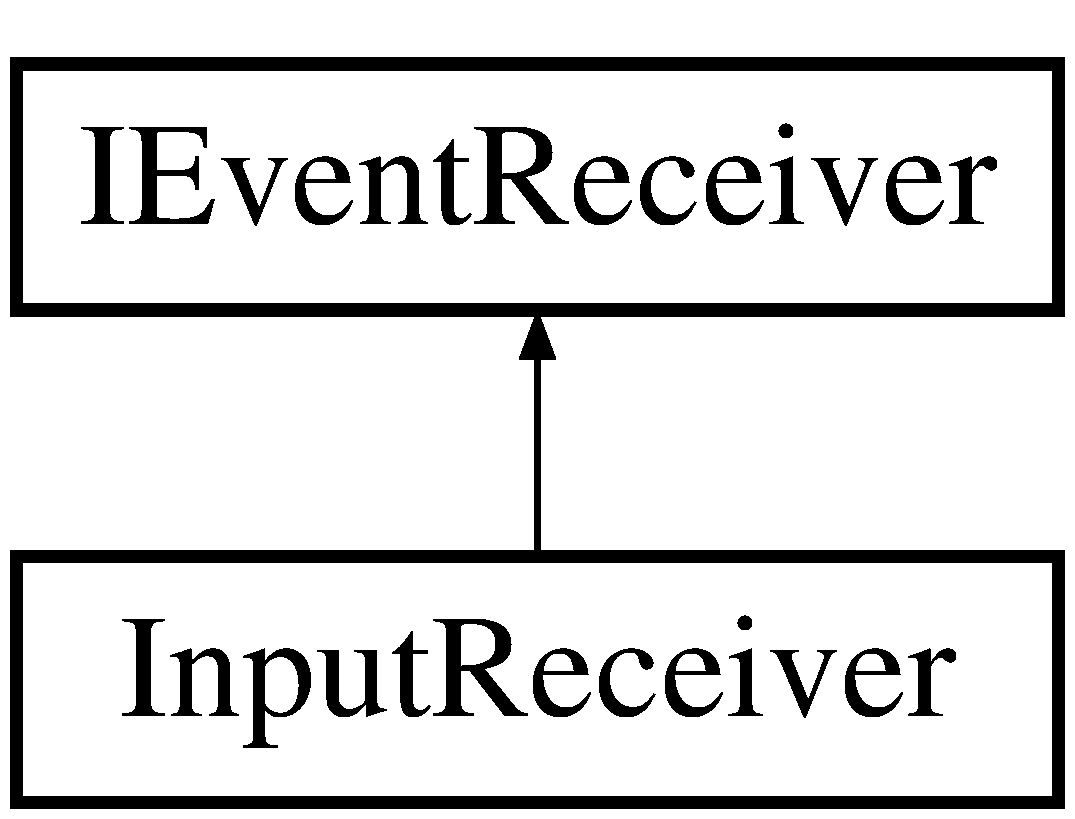
\includegraphics[height=2.000000cm]{class_input_receiver}
\end{center}
\end{figure}
\subsection*{Public Member Functions}
\begin{DoxyCompactItemize}
\item 
\mbox{\Hypertarget{class_input_receiver_a93d0cb79217595eb9bc29f5785bb5620}\label{class_input_receiver_a93d0cb79217595eb9bc29f5785bb5620}} 
irr\+::core\+::array$<$ irr\+::\+S\+Joystick\+Info $>$ {\bfseries Get\+Joystick\+Info} ()
\item 
\mbox{\Hypertarget{class_input_receiver_a0f4ecd33eace7fe2778cba699a06cd82}\label{class_input_receiver_a0f4ecd33eace7fe2778cba699a06cd82}} 
void {\bfseries Check\+Joystick\+Present} (irr\+::\+Irrlicht\+Device $\ast$device)
\item 
\mbox{\Hypertarget{class_input_receiver_a8cbad01c0e0dcaa953685b1c932d8ce6}\label{class_input_receiver_a8cbad01c0e0dcaa953685b1c932d8ce6}} 
bool {\bfseries On\+Event} (const irr\+::\+S\+Event \&event)
\item 
\mbox{\Hypertarget{class_input_receiver_a736d040738e9826b2abbcc0dd9cd085c}\label{class_input_receiver_a736d040738e9826b2abbcc0dd9cd085c}} 
bool {\bfseries Is\+Key\+Down} (irr\+::\+E\+K\+E\+Y\+\_\+\+C\+O\+DE key\+Code) const
\end{DoxyCompactItemize}
\subsection*{Static Public Attributes}
\begin{DoxyCompactItemize}
\item 
\mbox{\Hypertarget{class_input_receiver_a1763dd9cc9a31639592fb23115cdcc64}\label{class_input_receiver_a1763dd9cc9a31639592fb23115cdcc64}} 
static bool {\bfseries is\+Left\+Mouse\+Button\+Down} = false
\item 
\mbox{\Hypertarget{class_input_receiver_a4bffdbd7b8b83008a8f0d79ab018bb6b}\label{class_input_receiver_a4bffdbd7b8b83008a8f0d79ab018bb6b}} 
static irr\+::core\+::vector3df {\bfseries position} = core\+::vector3df(0,0,0)
\item 
\mbox{\Hypertarget{class_input_receiver_ad5486727fcb5faf69809b69f311c0b27}\label{class_input_receiver_ad5486727fcb5faf69809b69f311c0b27}} 
static irr\+::\+S\+Event\+::\+S\+Joystick\+Event {\bfseries joystick\+State}
\end{DoxyCompactItemize}
\subsection*{Private Attributes}
\begin{DoxyCompactItemize}
\item 
\mbox{\Hypertarget{class_input_receiver_a86ce1bb3b52f6bb3499224a508178f10}\label{class_input_receiver_a86ce1bb3b52f6bb3499224a508178f10}} 
bool {\bfseries key\+Is\+Down} \mbox{[}irr\+::\+K\+E\+Y\+\_\+\+K\+E\+Y\+\_\+\+C\+O\+D\+E\+S\+\_\+\+C\+O\+U\+NT\mbox{]}
\item 
\mbox{\Hypertarget{class_input_receiver_ab201d50024317b870b7020843033fd4a}\label{class_input_receiver_ab201d50024317b870b7020843033fd4a}} 
irr\+::core\+::array$<$ irr\+::\+S\+Joystick\+Info $>$ {\bfseries joystick\+Info}
\end{DoxyCompactItemize}


The documentation for this class was generated from the following files\+:\begin{DoxyCompactItemize}
\item 
D\+:/\+Documenten/\+S\+T\+U\+D\+I\+E G\+D/\+Game Engine/\+Irrlicht project/kommandos/Input\+Receiver.\+h\item 
D\+:/\+Documenten/\+S\+T\+U\+D\+I\+E G\+D/\+Game Engine/\+Irrlicht project/kommandos/Input\+Receiver.\+cpp\end{DoxyCompactItemize}

\hypertarget{class_level_generation}{}\section{Level\+Generation Class Reference}
\label{class_level_generation}\index{Level\+Generation@{Level\+Generation}}
\subsection*{Public Member Functions}
\begin{DoxyCompactItemize}
\item 
\mbox{\Hypertarget{class_level_generation_a3eebfed13225b555bd0530503908f4be}\label{class_level_generation_a3eebfed13225b555bd0530503908f4be}} 
void {\bfseries Place\+Arenas} (I\+Scene\+Manager $\ast$smgr, int max\+Arenas)
\end{DoxyCompactItemize}
\subsection*{Private Member Functions}
\begin{DoxyCompactItemize}
\item 
\mbox{\Hypertarget{class_level_generation_acf33a455315bb333e8d218a27ab00c2e}\label{class_level_generation_acf33a455315bb333e8d218a27ab00c2e}} 
void {\bfseries Place\+Doors} (I\+Scene\+Manager $\ast$smgr, core\+::array$<$ I\+Scene\+Node $\ast$$>$ arenas)
\end{DoxyCompactItemize}


The documentation for this class was generated from the following files\+:\begin{DoxyCompactItemize}
\item 
D\+:/\+Documenten/\+S\+T\+U\+D\+I\+E G\+D/\+Game Engine/\+Irrlicht project/kommandos/Level\+Generation.\+h\item 
D\+:/\+Documenten/\+S\+T\+U\+D\+I\+E G\+D/\+Game Engine/\+Irrlicht project/kommandos/Level\+Generation.\+cpp\end{DoxyCompactItemize}

\hypertarget{class_player}{}\section{Player Class Reference}
\label{class_player}\index{Player@{Player}}
\subsection*{Public Member Functions}
\begin{DoxyCompactItemize}
\item 
\mbox{\Hypertarget{class_player_ac207dd2957a2e3c4e734a9a074c2321d}\label{class_player_ac207dd2957a2e3c4e734a9a074c2321d}} 
{\bfseries Player} (irr\+::\+Irrlicht\+Device $\ast$device)
\item 
\mbox{\Hypertarget{class_player_ae9f5a597f15e29673c47abe47c3f1d79}\label{class_player_ae9f5a597f15e29673c47abe47c3f1d79}} 
void {\bfseries Take\+Damage} (irr\+::f32 damage)
\item 
\mbox{\Hypertarget{class_player_aa6cc636d92ca5ccba15a5af2ef7f224a}\label{class_player_aa6cc636d92ca5ccba15a5af2ef7f224a}} 
void {\bfseries Draw\+Health\+Bar} ()
\item 
\mbox{\Hypertarget{class_player_af8f50f5e8d8cb980959ba94655a0fcc1}\label{class_player_af8f50f5e8d8cb980959ba94655a0fcc1}} 
void {\bfseries Move} (irr\+::scene\+::\+I\+Scene\+Node $\ast$player\+Node, \mbox{\hyperlink{class_input_receiver}{Input\+Receiver}} input\+Receiver)
\end{DoxyCompactItemize}
\subsection*{Public Attributes}
\begin{DoxyCompactItemize}
\item 
\mbox{\Hypertarget{class_player_a83dd8a4ec58053dd77e3f5e3e9b8e26e}\label{class_player_a83dd8a4ec58053dd77e3f5e3e9b8e26e}} 
irr\+::core\+::vector3df {\bfseries current\+Position}
\end{DoxyCompactItemize}


The documentation for this class was generated from the following files\+:\begin{DoxyCompactItemize}
\item 
D\+:/\+Documenten/\+S\+T\+U\+D\+I\+E G\+D/\+Game Engine/\+Irrlicht project/kommandos/Player.\+h\item 
D\+:/\+Documenten/\+S\+T\+U\+D\+I\+E G\+D/\+Game Engine/\+Irrlicht project/kommandos/Player.\+cpp\end{DoxyCompactItemize}

%--- End generated contents ---

% Index
\backmatter
\newpage
\phantomsection
\clearemptydoublepage
\addcontentsline{toc}{chapter}{Index}
\printindex

\end{document}
